\section{Desarrollo}
	En la actualidad, algunos de los programas académicos de posgrado relacionados a los Sistemas Complejos son los siguientes:
\subsection{UACM - Maestría en Ciencias de la Complejidad}
	La Universidad de la Ciudad de México, ubicada en la Ciudad de México, ofrece una Maestría en Ciencias de la Complejidad\cite{UACM}. El plan de estudio elaborado para la misma se divide en dos grandes orientaciones
	\begin{enumerate}
		\item Opción A: Abarca temas como la construcción de modelos con herramientas de representación y análisis no lineal, interacción con profesionales de los campos de estudio de los procesos representados para juzgar la pertenencia de los mismos y se fomenta el trabajo interdisciplinario.
		\item Opción B: Se busca la comprensión del lenguaje, hipótesis y las limitaciones de los modelos, se busca que los estudiantes sean capaces de utilizar simuladores y apoyos computacionales para calibrar y juzgar la pertenencia de los modelos.
	\end{enumerate}

\subsection{El Colegio de Morelos - Maestría y Doctorado en Filosofía y Ciencia}
	El Colegio de Morelos, ubicado en Cuernavaca, Morelos, en colaboración con el Centro de Ciencias de la Complejidad de la UNAM, oferta una Maestría y un Doctorado  en Filosofía y Ciencia\cite{MORELOS}.

	En este programa se estudia la naturaleza de los sistemas complejos en el ámbito económico, político y socioambiental, buscando la resolución de los problemas globales desde un enfoque transdisciplinario.

\subsection{Instituto Balseiro - Maestría en Ciencias Físicas}
	El Instituto Balseiro localizado en San Carlos de Bariloche Río Negro, Argentina, oferta una Maestría en Ciencias Físicas, la cual ofrece la posibilidad de orientarse a los sistemas complejos\cite{Balseiro}.

	La orientación tiene como objetivo formar formar un profesional compenetrado con las posibles aplicaciones interdisciplinarias de la física estadística de sistemas fuera de equilibrio, y capacitarlos para encarar ámbitos de investigación básica y aplicada.

\subsection{CCSS - Carrera Universitaria con especialidad en Sistemas Complejos/Maestría en Sistemas Complejos}
	La Universidad de Utrecht, ubicada en Holanda, tiene un Centro de Estudio para los Sistemas Complejos (CCSS por sus siglas en inglés), en el cual se ofertan una carrera universitaria con especialidad en sistemas complejos\cite{CCSS} al igual que ofertan una Maestría en Sistemas Complejos.

	Cabe señalara que ambas son impartidas en el CCSS, en el caso de la carrera universitaria el objetivo de la misma es formar a los estudiantes y darles la oportunidad de ganar conocimiento en conceptos como emergimiento, auto-dirección y adaptación. La interdisciplina juega un papel importante en esta especialidad.

	% \begin{figure}[H]
	% 	\begin{center}
	% 		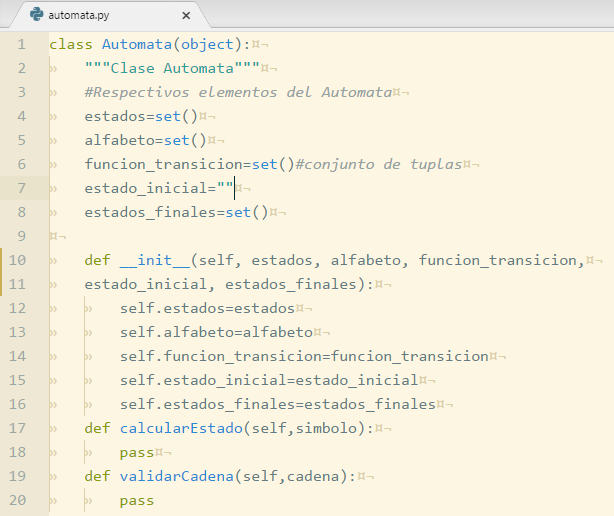
\includegraphics[width=15cm, height=12cm]{img/automata.png}
	% 		\caption{automata.py}
	% 		\label{fig:tablas}
	% 	\end{center}
	% \end{figure}